\documentclass[unicode]{beamer}
\usetheme{Madrid}
\usecolortheme{seahorse}     %цветовая схема
\useinnertheme{circles}   %внутренняя тема
\usefonttheme{serif}    %шрифты

\usepackage[utf8]{inputenc}
\usepackage[T2A]{fontenc}
\usepackage[russian]{babel}
\usepackage[listings,theorems]{tcolorbox}
\usepackage{caption}
\usepackage[labelsep=period]{caption}
\setbeamertemplate{caption}[numbered]
\graphicspath{{../LaTeX/pic}}

\definecolor{shBlue}{HTML}{d6d6f0}
\definecolor{lightGray}{HTML}{F5F5F5}
\definecolor{spGreen}{HTML}{93DDC2}
\definecolor{spBlue}{HTML}{007AFF}
\definecolor{mainBackground}{HTML}{F9FEFC}

\makeatletter
\newcommand*{\rom}[1]{\expandafter\@slowromancap\romannumeral #1@}
\makeatother


\setbeamercolor{block title}{bg=shBlue!70,fg=black}
\setbeamercolor{block body}{bg=lightGray!50,fg=black}
% \setbeamercolor{frametitle}{fg=selected,bg=spGreen}
% \setbeamercolor{background canvas}{bg=mainBackground}
\setbeamertemplate{blocks}[rounded][shadow=false]

\title[Курсовая работа]{Модель термоупругого разрушения хрупкого материала}
\author[Токарев~А.И.]{Токарев~А.И.}
\institute[]{МГТУ им. Н.Э. Баумана}
\date{\today}

\begin{document}

    \begin{frame}
        \titlepage
    \end{frame}

    \begin{frame}
        \frametitle{Содержание}
        \tableofcontents
    \end{frame}

    \section{Постановка задачи}

    \begin{frame}
        \frametitle{Постановка задачи}
        \begin{block}{Тензор малых деформаций Коши}
            \fontsize{10.4pt}{12pt}\selectfont
            Деформации -- смещение каждой точки тела. Тензор деформаций симметричен и может быть записан следующим образом:
            \[
                \varepsilon_{kl} = \dfrac{1}{2}\Bigl( \dfrac{\partial u_k}{\partial x_l} + \dfrac{\partial u_l}{\partial x_k} \Bigr) = \varepsilon_{kl}^e +  \varepsilon_{kl}^0, \quad k, l = 1, 2, 3,  
            \]
            \noindent где $\varepsilon_{kl}^e$ -- упругие деформации; $\varepsilon_{kl}^0$ -- неупругие деформации.
        \end{block}

        \begin{block}{Тензор напряжений}
            \fontsize{10.4pt}{12pt}\selectfont
            Напряжения и деформации связаны линейно соотношением:
            \[
                \sigma_{ij} = C_{ijkl} \varepsilon_{kl}^e = C_{ijkl}(\varepsilon_{kl} - \varepsilon_{kl}^0),
            \]
            \noindent $C_{ijkl}$ -- тензор упругих постоянных (четвертого ранга), в общем случае состоящий из $36$ компонент. 
        \end{block}
    \end{frame}

    \begin{frame}
        \begin{block}{}
            Для изотропного тела с учетом нотации Фойгта тензор упругих постоянных может быть преобразован к матрице $6$x$6$ с компонентами:
            \[
                \begin{pmatrix}
                    \lambda + 2\mu & \lambda & \lambda & 0 & 0 & 0 \\
                    \lambda & \lambda + 2\mu & \lambda & 0 & 0 & 0 \\
                    \lambda & \lambda & \lambda + 2\mu & 0 & 0 & 0 \\
                         0 &      0 &      0 & \mu & 0 & 0 \\
                         0 &      0 &      0 & 0 & \mu & 0 \\
                         0 &      0 &      0 & 0 & 0 & \mu \\
                  \end{pmatrix} 
            \]
        \end{block}

        \begin{block}{Уравнение равновесия}
            \fontsize{10.4pt}{12pt}\selectfont
            \[
              \dfrac{\partial \sigma_{ji}}{\partial x_j} + b_i = 0, \quad i,j = 1, 2, 3.
            \]
        \end{block}
    \end{frame}

    \section{Математическая модель для одномерного случая}
    \begin{frame}        
        \frametitle{Математическая модель для одномерного случая}
        \begin{block}{Аппроксимация}
            \[
              \dfrac{\sigma}{\sigma_f} = A + B e^{-C \tfrac{\varepsilon}{\varepsilon_f}},
            \]
            \noindent где коэффициенты A, B выводятся экспериментально. Для дикосида урана:
            $
              A = -0.024,\, B = 1.69, \, C = 0.5.  
            $
        \end{block} 
        \begin{figure}
            \centering
            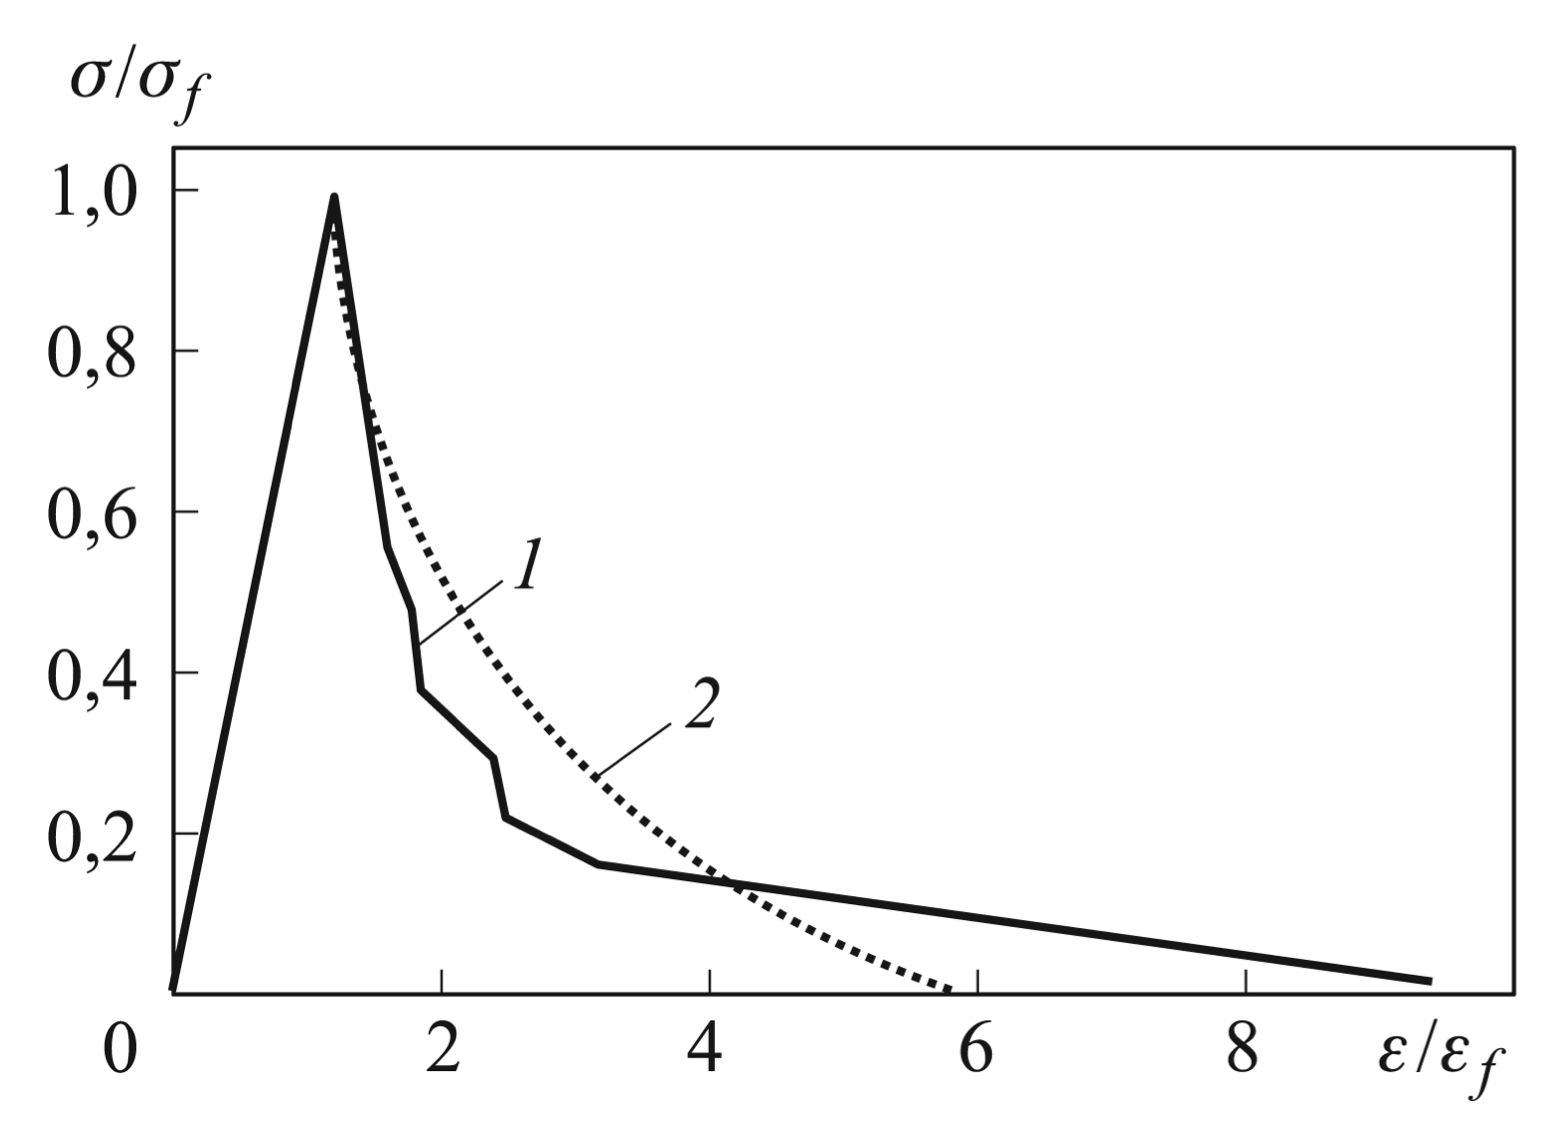
\includegraphics[width=0.4\textwidth]{ceramic.jpeg}
            \caption{Экспериментально выведенная зависимость напряжений от деформаций}
        \end{figure}
    \end{frame}

    \begin{frame}
        До достижения предела прочности $\sigma = \sigma_f^v$ тело ведет себя, как линейно-упругое. В области послепиковых значений деформаций и напряжений (инициализация трещины) просиходит разгрузка по нелинейному закону. 

        \vspace{0.7em}

        \begin{block}{Зависимость напряжений от деформаций}
            \[
                \sigma(\varepsilon) = 
                    \begin{cases}
                    E\varepsilon^e, & E\varepsilon^e < \sigma_f^v(\varepsilon); \\
                    \sigma_f \Bigl( A + B e^{-C \tfrac{\varepsilon^e}{\varepsilon_f}} \Bigr), & E\varepsilon^e \geq \sigma_f^v(\varepsilon),
                    \end{cases}
                \label{sigma}
            \]
            \noindent где $\sigma_f^v$ -- переменный предел прочности. 
        \end{block}

        \vspace{0.7em}

        Тело подвержено тепловым нагрузкам, описываемыми уравнением:
        \[
          T(x,t) = \tilde{T} + F(x)\tau(t),  
        \]
        \noindent тут $\tilde{T}$ -- средняя температура; $F(x)$ -- пространственное распределение температуры, а $\tau(x)$ -- временное.
    \end{frame}

    \begin{frame}
        Пусть $l$ -- длина стержня. Стержень закреплен с обоих концов, поэтому наложим некоторые ограничения:
        \[
          u(0, t) = u(l, t)  
        \]

        \begin{block}{Математическая модель}
            \[
                \begin{cases}
                    T(x, t) = \widetilde{T} + F(x) \tau(t), & t \geq 0, \quad 0 \leq x \leq l, \\[0.7em]
                    \dfrac{\partial \sigma}{\partial x} = 0, & 0 \leq x \leq l, \\[0.7em]
                    \sigma = \sigma(\varepsilon - \varepsilon^T), & \varepsilon = \dfrac{\partial u}{\partial x}, \quad \varepsilon^T = \alpha(T - T_0), \\[0.7em]
                    u(0, t) = u(l, t) = 0.
                  \end{cases}  
            \]
        \end{block}
    \end{frame}

    \section{Алгоритм}
    \begin{frame}
        \frametitle{Алгоритм}
            \begin{enumerate}
                \item В предположении линейной упругости решаем уравнение равновесия и находим деформации в каждой точке сетки:
                \[
                    \dfrac{\partial \sigma}{\partial x} = \dfrac{\partial (E (\varepsilon - \varepsilon^t))}{\partial x} = 0.
                \]
                \item Если то, то се, если се, то то.
                \item Пятое десятое
                \item Ну и еще что-то
            \end{enumerate}
    \end{frame}

    \section{Пример}
    \begin{frame}
        \frametitle{Пример}
        Рассмотрим процесс разрушения наглядно. Построим графики зависимости: напряжений от деформаций $\sigma(\varepsilon - \varepsilon^T)$; деформаций и напряжений от времени $\varepsilon(t), \, \sigma(t)$ и температуры от времени $T(t)$.

        \vspace{0.7em}

        \begin{block}{Условия}
            Определим зависимость температуры от координаты и времени:
            \[
                T(x, t) = \widetilde{T} + F(x) t \sin t, \quad F(x) = a \sin \Bigl( \dfrac{\pi x}{l} \Bigr). 
            \]

            Для линейного случая зависимости можно найти аналитическое решение для перемещений:
            \[
                u(x, t) = \dfrac{a l t \alpha \sin(t) - 2 a t x \alpha \sin(t) - a l t \alpha \cos (\tfrac{\pi x}{l}) \sin t}{\pi}.
            \]
        \end{block}
    \end{frame}

    \begin{frame}
        \begin{figure}
            \centering
            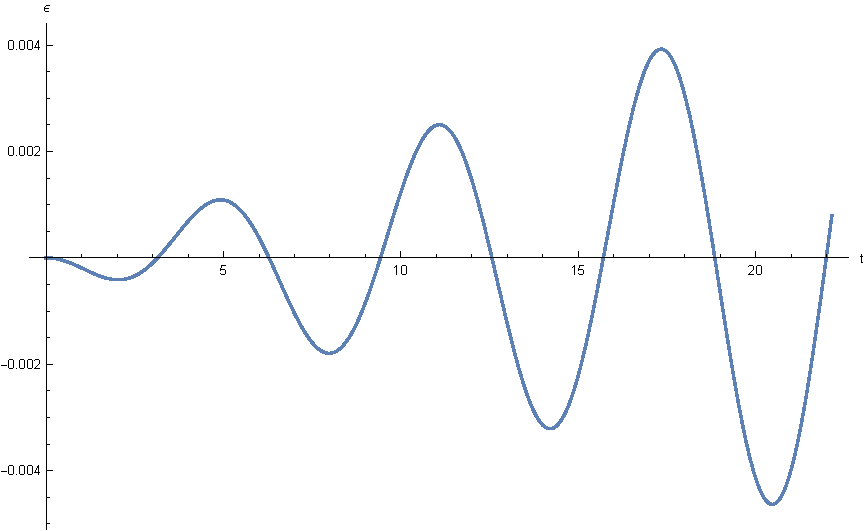
\includegraphics[width=0.45\textwidth]{T1/h_1_tau_0.05/epsilon(t).pdf}
            \caption{Зависимость деформаций от времени}
        \end{figure}

        \begin{figure}
                \centering
                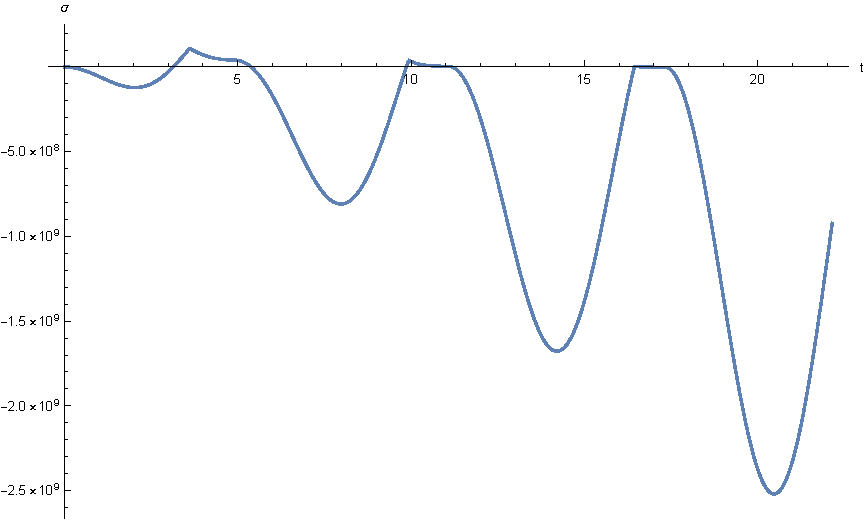
\includegraphics[width=0.45\textwidth]{T1/h_1_tau_0.05/sigma(t).pdf}
                \caption{Зависимость напряжений от времени}
       \end{figure}
    \end{frame}

    \begin{frame}
        \begin{figure}
            \centering
            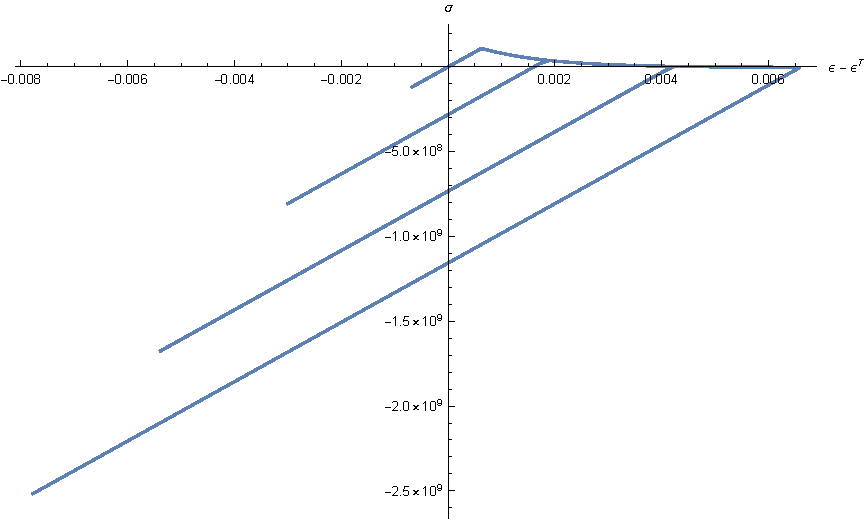
\includegraphics[width=0.45\textwidth]{T1/h_1_tau_0.05/sigma(epsilon).pdf}
            \caption{Зависимость напряжений от деформаций}
        \end{figure}

        \begin{figure}
                \centering
                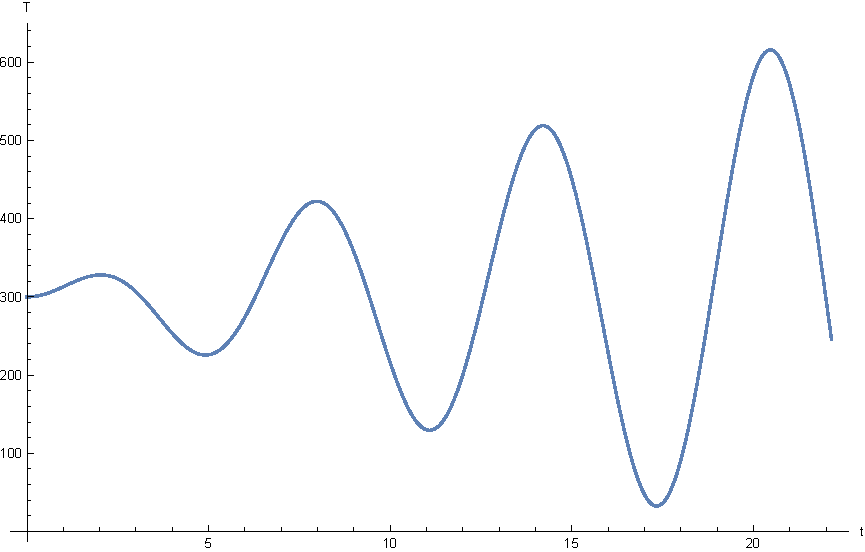
\includegraphics[width=0.45\textwidth]{T1/h_1_tau_0.05/T(t).pdf}
                \caption{Зависимость температуры от времени}
       \end{figure}
    \end{frame}
    

    \begin{frame}
        \frametitle{Список использованных источников}
        \begin{thebibliography}{9}
            \bibitem{Karelia} Тензоры напряжений и деформаций. URL: \url{http://solidstate.karelia.ru/p/tutorial/ftt/Part4/part4_1.htm}

            \bibitem{Deform} Тензор деформаций. SolverBook - онлайн сервисы для учебы. URL: \url{http://ru.solverbook.com/spravochnik/fizika/tenzor-deformacii/}

            \bibitem{Flex} Теория упругости. Wikipedia –- свободная энциклопедия. URL: \url{https://en.wikipedia.org/wiki/Linear_elasticity}

             \bibitem{Galanin} Галанин М.П. Методы численного анализа математических моделей/М.П. Галанин, Е.Б. Савенков.–М. : Изд-во МГТУ им. Н.Э. Баумана, 2010.–591, [1] с.: ил. (Математическое моделирование в технике и технологии)

        \end{thebibliography}
    \end{frame}

    \begin{frame}
        \frametitle{Список использованных источников}
        \begin{thebibliography}{9}

            \bibitem{GalaninAndOthers} Математическое моделирование разрушения хрупкого материа- ла под действием тепловых нагрузок / М.П. Галанин [и др.] // Препринты ИПМ им. М.В. Келдыша. 2013.No 100. 36 с. URL: \url{http://library.keldysh.ru/preprint.asp?id=2013-100}
        \end{thebibliography}
    \end{frame}
    


\end{document}